\documentclass[]{beamer}
% \geometry{papersize={16cm,9.60cm}}
\usepackage{etex}
\usepackage{amsmath}
\usepackage{tikz}
\usepackage{multimedia}
\usetheme{Boadilla}
\usepackage{graphicx}
%\usepackage{inputenc}

% \mode<presentation>
% {
%   \usetheme{default}
%   \setbeamercovered{transparent}
% }


% {\vskip5pt}

%% customize layout, bullet points navigation toolbar
\setbeamertemplate{navigation symbols}{}%remove navigation symbols
\setbeamertemplate{enumerate items}[default]
\setbeamertemplate{navigation symbols}{}
\setbeamertemplate{itemize items}[circle]
\setbeamercolor{enumerate item}{fg=black}

\setbeamertemplate{footline}{}
\setbeamersize{text margin left = 2.0em}
\setbeamersize{text margin right = 2.0em}

\usepackage{times}
\usepackage[T1]{fontenc}

% Or whatever. Note that the encoding and the font should match. If T1
% does not look nice, try deleting the line with the fontenc.

\setbeamertemplate{navigation symbols}{}

\title{ Cognitive (Neuro) Psychology }
\subtitle{III. Pattern vision}
\author{ Marianne Maertens }
\institute[TU Berlin]{Technische Universit\"at Berlin}
\date{July 2016}

\begin{document}
\setbeamertemplate{enumerate items}[default]
\setbeamertemplate{headline}

\frame{\titlepage}

\AtBeginSection[]
{
  \begin{frame}<beamer>
    \frametitle{Layout}
    \tableofcontents[currentsection]
  \end{frame}
}

\begin{frame}
 \frametitle{Cortical visual pathways}
 \begin{center}
\includegraphics<1>[width=110mm]{figs/l3/cortical_pathways.png}
 \end{center}
\end{frame}


\begin{frame}
 \frametitle{Path of image processing: eye to brain}
\begin{columns}[T]
 \begin{column}{40mm}
  \begin{itemize}
  \setlength{\itemsep}{5pt}
   \item<1-> eye
   \item[]
   \item<2-> lateral geniculate nucleus LGN
   \item<2-> primary visual cortex V1
  \end{itemize}
 \end{column}

 \begin{column}{70mm}
  \includegraphics<1>[width=70mm]{figs/l3/retina_info_flow.png}
  \includegraphics<2>[width=70mm]{figs/l3/cortical_pathways2.png}
 \end{column}
\end{columns}
\end{frame}


\begin{frame}
\frametitle{Basic visual functions: Acuity}
\begin{overlayarea}{110mm}{60mm}
  \begin{center}
\includegraphics<1>[width=110mm]{figs/l3/ori_acuity_demo.png}
\includegraphics<2>[width=30mm]{figs/l3/ori_acuity_demo.png}
 \end{center}
\end{overlayarea}
\only<1->{Acuity: the smallest spatial detail that can be resolved}
\end{frame}


\begin{frame}
\frametitle{How to measure acuity?}
\begin{overlayarea}{110mm}{60mm}
Visual angle of one cycle of the grating 
\begin{itemize} 
 \item[]
 \item $atan(\frac{size}{distance}) = atan(\frac{2}{6500})=.017$
\end{itemize}
  \begin{center}
\includegraphics<1>[width=80mm]{figs/l3/visual_angle.png}
 \end{center}
\end{overlayarea}
\end{frame}

\begin{frame}
\frametitle{How to measure acuity?}
\begin{overlayarea}{110mm}{60mm}
Snellen \textbf{E} test
\begin{itemize} 
 \item eye doctors use distance to characterize acuity
 \item "20/20 vision" your distance/normal vision distance
\end{itemize}
  \begin{center}
\includegraphics<1>[width=50mm]{figs/l3/snellen_E.png}
 \end{center}
\end{overlayarea}
\end{frame}

\begin{frame}
\frametitle{Resolution acuity limits spatial vision}
  \begin{center}
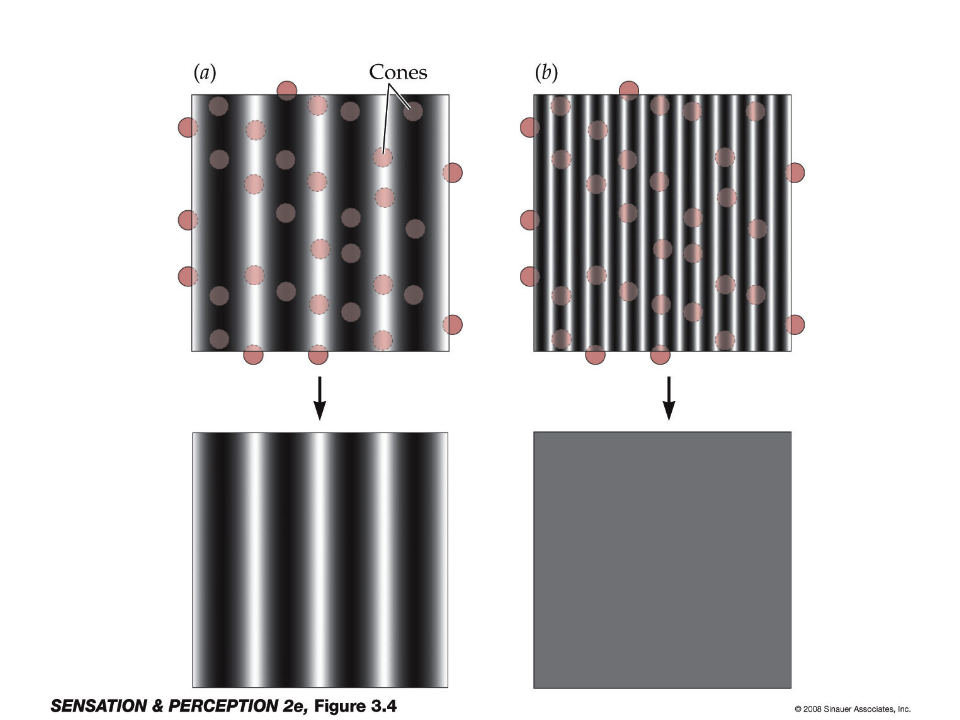
\includegraphics[width=100mm]{figs/l3/grating_sampling.png}
 \end{center}
\end{frame}


\begin{frame}
\frametitle{Acuity for low contrast stimuli}
\begin{overlayarea}{110mm}{80mm}
\begin{itemize}
 \item Contrast
\end{itemize}
\begin{columns}[T]
 \begin{column}{15mm}

\includegraphics[width=15mm]{figs/l3/high_contrast.jpg}


\includegraphics[width=15mm]{figs/l3/medium_contrast.jpg}
\end{column}

 \begin{column}{50mm}
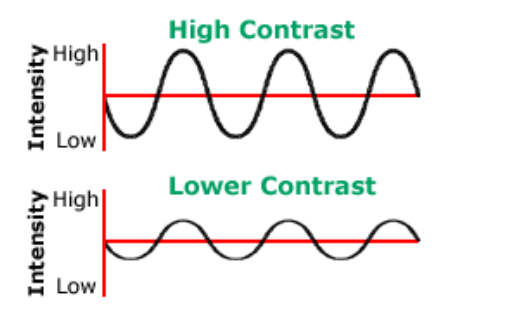
\includegraphics[width=50mm]{figs/l3/sine_wave_high_low.png}
 \end{column}
\end{columns}

\begin{itemize}
 \item Spatial frequency
\end{itemize}

\begin{center}

\includegraphics[width=90mm]{figs/l3/gabors_sf.png}
\end{center}
\end{overlayarea}
\end{frame}


\begin{frame}
\frametitle{Contrast Sensitivity Function - CSF}
\begin{center}
\includegraphics<1>[width=100mm]{figs/l3/csf_diagram.png}
\includegraphics<2>[width=100mm]{figs/l3/csf_demo.png}
\end{center}
\end{frame}
% 
% \begin{frame}
%  \begin{exampleblock}{Thinking}
% You cannot observe atoms directly. We still think they
% exist. Why? We cannot observe thoughts in other people
% directly. We still think they exist. Why?
%  \end{exampleblock}
% \end{frame}


\begin{frame}
 \frametitle{Retinal ganglion cell responses to stripes}
\begin{itemize}
 \item sensitivity to spatial frequency
\end{itemize}

\begin{center}
\includegraphics<1>[width=80mm]{figs/l3/lgn_gratings.png}
\end{center}
\end{frame}

\begin{frame}
 \frametitle{Detour - single cell recordings}
\begin{itemize}
 \item recordings of action potentials in monkeys
 \item ``spike'' counts 
\end{itemize}


\begin{columns}[T]
 \begin{column}{40mm}
\begin{center}
\includegraphics<1>[width=40mm]{figs/l3/ward_single_cell_recording.png}
\end{center}
 \end{column}

 \begin{column}{40mm}
\vspace{5mm}
\begin{center}
\includegraphics<1>[width=40mm]{figs/l3/single_cell_electrode.png}
\end{center}
 \end{column}

 \begin{column}{20mm}
\vspace{10mm}
\begin{center}
\includegraphics<1>[width=20mm]{figs/l3/spike_counts.png}
\end{center}
 \end{column}
\end{columns}
\end{frame}



\begin{frame}
 \frametitle{Retinal ganglion cell responses to stripes}
\begin{itemize}
 \item sensitivity to spatial frequency
\end{itemize}

\begin{center}
\includegraphics<1>[width=80mm]{figs/l3/lgn_gratings.png}
\end{center}
\end{frame}


\begin{frame}
 \frametitle{Retinal ganglion cell responses to stripes}
\begin{itemize}
 \item sensitivity to spatial phase
\end{itemize}

\begin{center}
\includegraphics<1>[width=80mm]{figs/l3/lgn_phase.png}
\end{center}
\end{frame}


\begin{frame}
 \frametitle{Down the visual pathway}
\begin{center}
\includegraphics<1>[width=80mm]{figs/l3/cortical_pathways2.png}
\end{center}
\end{frame}



\begin{frame}
 \frametitle{The Lateral Geniculate Nucleus - LGN}
\begin{overlayarea}{113mm}{69mm}
\begin{columns}[T]
 \begin{column}{50mm}
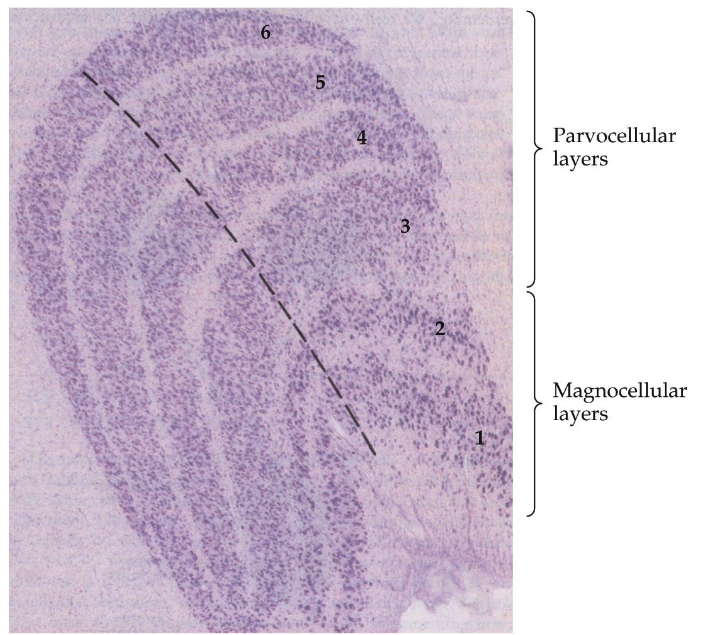
\includegraphics[width=60mm]{figs/l3/lgn_layers.png}
 \end{column}

 \begin{column}{60mm}
\begin{itemize}
 \setlength{\itemsep}{5pt}
 \item parvocellular layers - details of stationary targets
 \item[]
 \item magnocellular layer - large, fast-moving objects
\end{itemize}
 \end{column}
\end{columns}
\end{overlayarea}
\end{frame}

\begin{frame}
 \frametitle{The Lateral Geniculate Nucleus - LGN}
\begin{columns}[T]
 \begin{column}{60mm}
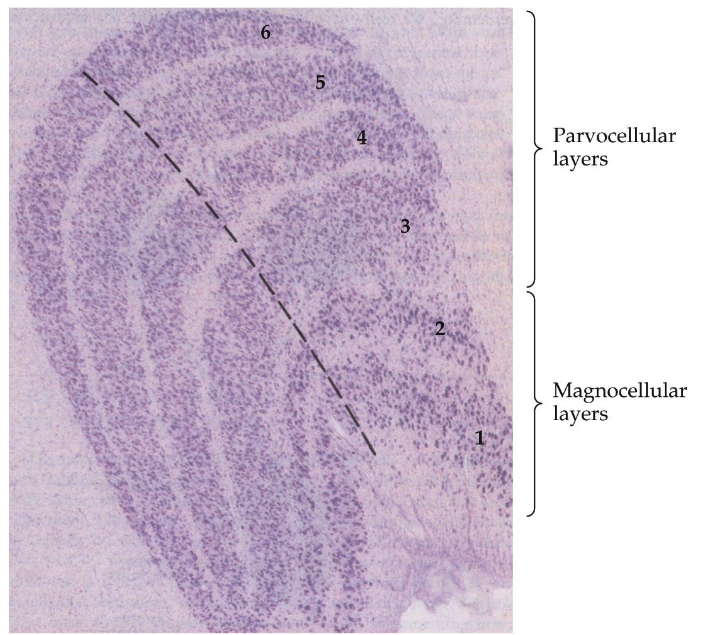
\includegraphics[width=60mm]{figs/l3/lgn_layers.png}
 \end{column}

 \begin{column}{50mm}
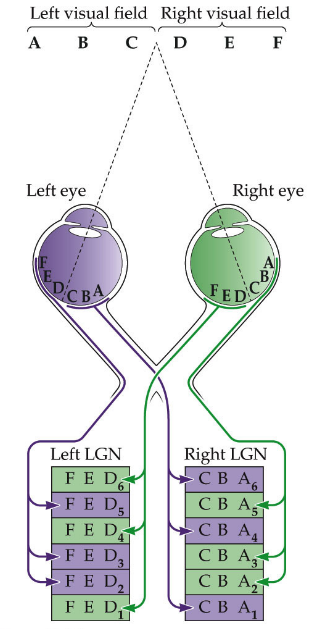
\includegraphics[width=35mm]{figs/l3/visual_field_lgn.png}
 \end{column}
\end{columns}
\end{frame}

\begin{frame}
 \frametitle{Down the visual pathway}
\begin{center}
\includegraphics<1>[width=80mm]{figs/l3/cortical_pathways2.png}
\end{center}
\end{frame}



\begin{frame}
 \frametitle{The Primary Visual Cortex - V1}
\begin{overlayarea}{113mm}{69mm}
\begin{columns}[T]
 \begin{column}{50mm}
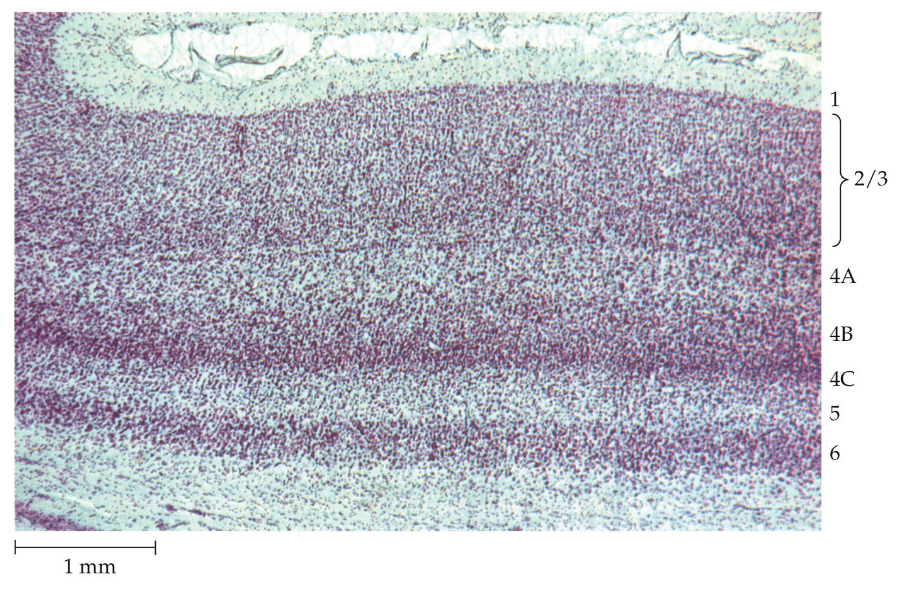
\includegraphics[width=60mm]{figs/l3/v1_layers.png}
 \end{column}

 \begin{column}{60mm}
\begin{itemize}
 \setlength{\itemsep}{5pt}
 \item[]
 \item[]
 \item[]
 \item parvocellular layers - 4C$\beta$
 \item magnocellular layer - 4C$\alpha$
\end{itemize}
 \end{column}
\end{columns}
\end{overlayarea}
\end{frame}


\begin{frame}
 \frametitle{The Primary Visual Cortex - V1}
\begin{itemize}
 \item<1> Topography and magnification
\end{itemize}

\begin{center}
\includegraphics<1>[width=60mm]{figs/l3/magnification_topography.png}
\includegraphics<2>[width=100mm]{figs/l3/snellen_magnification.png}
\end{center}
\end{frame}

\begin{frame}
 \frametitle{V1 neurons are orientation selective}
\begin{columns}[T]
 \begin{column}{55mm}
\begin{center}
\includegraphics<1->[width=50mm]{figs/l3/ori_tuning.png}
\end{center}
 \end{column}

 \begin{column}{55mm}
\begin{center}
\includegraphics<2>[width=50mm]{figs/l3/simple_cell_model.png}
\end{center}
 \end{column}
\end{columns}
\end{frame}


\begin{frame}
 \frametitle{Simple and complex cells in V1}
\begin{overlayarea}{110mm}{70mm}
\begin{columns}[T]
 \begin{column}{55mm}
\centering{Simple}
\begin{center}
\includegraphics<1->[width=50mm]{figs/l3/odd_even_simple_cells.png}
\end{center}
 \end{column}

 \begin{column}{55mm}
\centering{Complex}
\begin{center}
\includegraphics<2->[width=50mm]{figs/l3/complex_cell_response.png}
\end{center}
 \end{column}
\end{columns}

\only<3->{
\begin{center}
\centering{End-stopped}

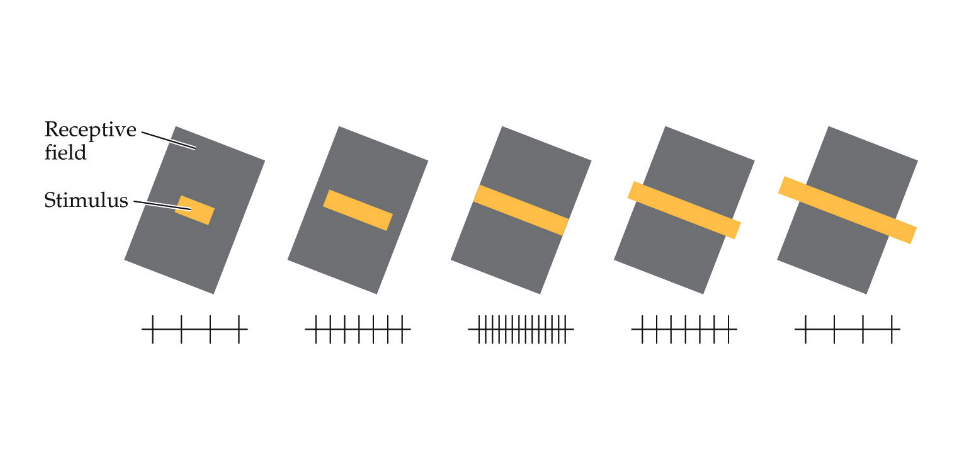
\includegraphics[width=50mm]{figs/l3/end_stopped_cell_response.png}
\end{center}
}
\end{overlayarea}
\end{frame}


\begin{frame}
 \frametitle{Selective adaptation: the psychologist's electrode}
\begin{center}
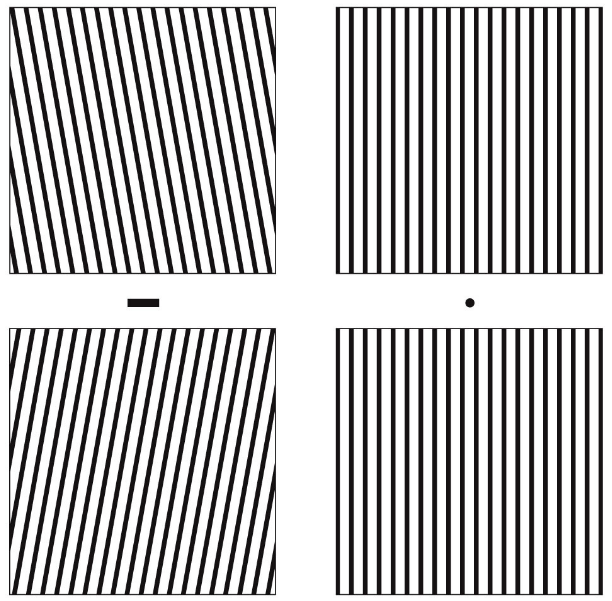
\includegraphics[width=70mm]{figs/l3/ori_tilt_aftereffect.png}
\end{center}
\end{frame}

\begin{frame}
 \frametitle{Selective adaptation: the psychologist's electrode}
\begin{overlayarea}{110mm}{80mm}
\begin{columns}[T]
\begin{column}{50mm}
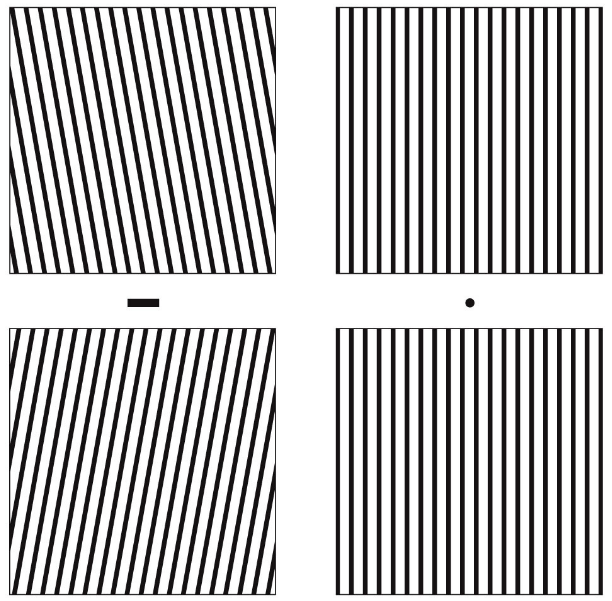
\includegraphics[width=50mm]{figs/l3/ori_tilt_aftereffect.png}
\end{column}
 
\begin{column}{60mm}
\includegraphics<1>[width=50mm]{figs/l3/ori_pre_adaptation_0.png}

\includegraphics<2->[width=50mm]{figs/l3/ori_pre_adaptation.png}

\includegraphics<1>[width=50mm]{figs/l3/ori_tuning.png}
 
\includegraphics<3>[width=50mm]{figs/l3/ori_post_adaptation.png}
\end{column}
\end{columns}
\end{overlayarea}
\end{frame}


\begin{frame}
 \frametitle{Selective adaptation: the psychologist's electrode}
\begin{overlayarea}{110mm}{80mm}
\begin{columns}[T]
\begin{column}{45mm}
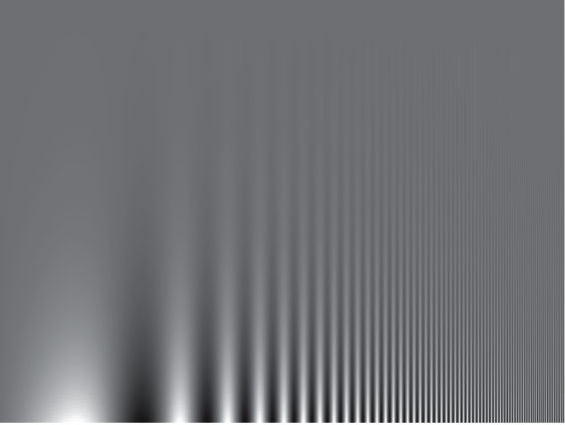
\includegraphics[width=45mm]{figs/l3/sf_adaptation_test.png}
\end{column}
 
\begin{column}{45mm}
\includegraphics<1,4->[width=45mm]{figs/l3/sf_adaptation_vert.png}

\includegraphics<2>[width=45mm]{figs/l3/sf_adaptation_csf.png}

\includegraphics<3>[width=45mm]{figs/l3/sf_adaptation_hori.png}
\end{column}
\end{columns}

\begin{center}
\includegraphics<4>[width=110mm]{figs/l3/sf_adaptation.png}
\end{center}
\end{overlayarea}
\end{frame}

\begin{frame}
 \frametitle{Spatial frequency tuned pattern analyzers in human vision}
\begin{center}
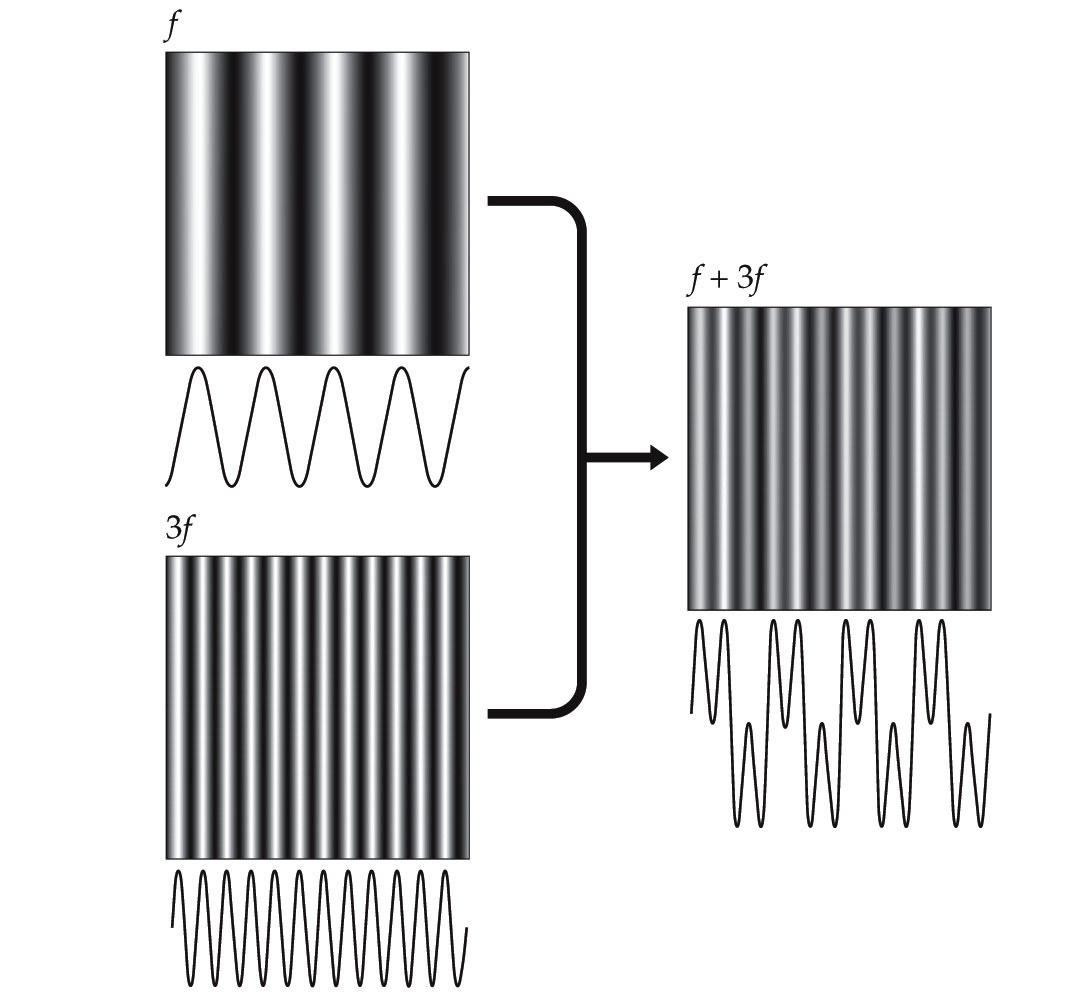
\includegraphics[width=70mm]{figs/l3/graham_nachmias.jpg}
\end{center}
\end{frame}


\begin{frame}
 \frametitle{Summary}
\begin{itemize}
\setlength{\itemsep}{5pt}
 \item 
 \item 
 \item 
 \item 
\end{itemize}

\end{frame}




\begin{frame}
 \frametitle{References}
\begin{small}
\begin{itemize}
 \item  Wolfe, J.M., Kluender, K.R. \& Levi, D.M. (2012).\textit{Sensation \& Perception}. Sinauer Associates: Sunderland, MA. 
 \item 
\end{itemize}
\end{small}
\end{frame}


\end{document}